\documentclass[../main.tex]{subfiles}
\graphicspath{ {../img/} }


\begin{document}


	\chapter{Our choice and design}

    \section{What make us choose a botnet}

    When we began to work on the project, we first had to choose a good project.
    Many other choose to make a website or something related, but we were more interested in cybersecurity related stuff.
    That why, our first idea was to make a honypot.
    But the problem was that soon enough, we realise that we couldn't get any good ideas, or realisables ideas in the time we had.
    Because of that, we decided to change.
    We thought, what if we decided to make a malware?
    Our first idea was to make a software, with a backdoor inside.
    But the backdoor is for doing what?
    We choosed to add it to a botnet.
    As the project matured, we decided to not making the backdoor, bot only the botnet, and the way it will be ran will be by a remote code execution exploit. 
    % TODO: Choose the references we used to reaserch the perfect malware, and add it to the references.


	\vspace{10pt}

    \section{Plan and idea of the botnet}

    The first part of every project, when we know what project we want to make, is to design it.
    We first choosed, the languaged that we were supposed to use.
    We choosed RUST.
    It's a fast language like C, but everytime you compile, it gives you some tips on how to solves problems in your code.
    It's other big advantage is that it's a modern language, with a lot of modern feature, and constantly check that there is no problem with the memory allocation.
    None of us is a experienced developper, as such, learning rust was the most adapted thing we could made for the project.
    After that, we made a list of the differents parts of our project.

    \begin{itemize}

        \item sandboxed environment to avoid it to spread

        \item find an exploit to use

        \item make the actual botnet

        \item find a way to make the exploit run the botnet.

    \end{itemize}

    \vspace{10pt}

    \section{design explanations about the botnet.}

    \subsection{about the sanboxed environment}

    The first part for this project to run properly was to make the sandboxing environment.
    Fortunately, to makes one isn't that difficult. 
    We decided to use qemu, and make three mode.
    First, the instalation mode, use to install the linux system on an image.
    Second, the networking mode, or maintenance mode, use to install our botnet, or the software which contain the vulnerability.
    Lastly, the sandboxed mode, use for when we will actually run our botnet.

    \vspace{10pt}

    \subsection{how the botnet will be supposed to work}

    Our way to make it works is from a simple basic.
    We planned to make juste a server and a client.
    The server will have three role.
    1st, deliver the exploit to gain 5 bots.
    2nd, deliver command to thoses bots whenever they asks to do something.
    3rd, deliver it's own code to self replicate.

    The client, run by the exploit on the victim machine will do;
    1st, connect to the server to get the list of the files to download.
    2nd, download the files from the server to became a full node.
    3rd, launch another server, to become a node by itself.
    4th, at the same time as running the server, every 12h, get from the node parent the order file, execute the order, and make it available to the lowers nodes.

    A fully devellopped botnet should look like this.

    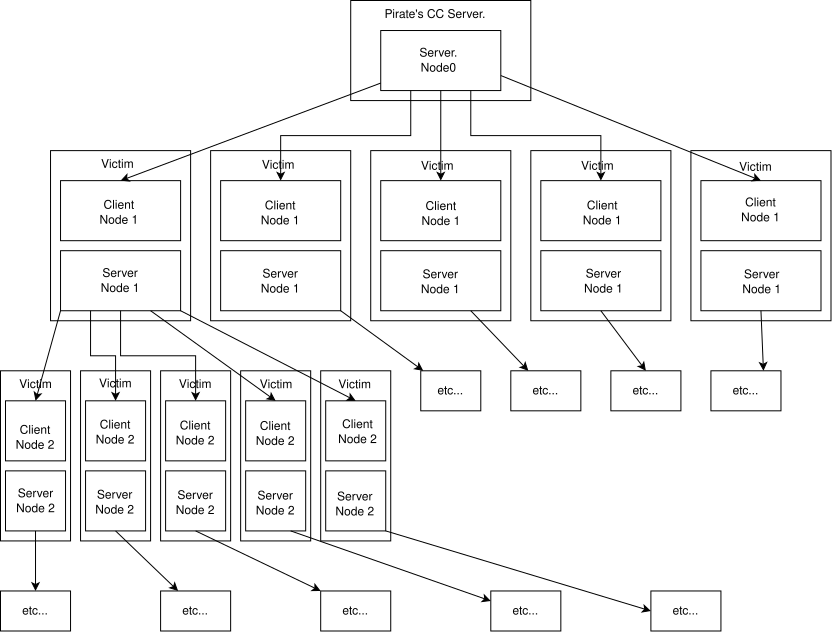
\includegraphics[width=450pt]{botnet.png}




\end{document}
